\section{Solution}
% arch start
\subsection{Architecture}
In this section we have used design by intuition to create the overall architecture of our system. Our argument for doing so is because we lack domain knowledge with using a tool as the one we are about to create. We will only gain this knowledge after we have spent time working on our first implementations of the DSL. Hopefully the development process will guide us to a more defined and fit for purpose architecture.

\subsubsection{Logical View}
Most of the objectives listed in the Objectives section(p.\pageref{sec:objectives}) are concerned with the ability of implementing the Diffie-Hellman-Merkle key exchange protocol. For our architecture we want to be more general in which protocol we implement. We will focus on creating a foundation for implementing an arbitrary protocol. Afterwards we will see if we need to add or change features to be able to implement a more complex protocol.

\begin{figure}[h]
	\centering
	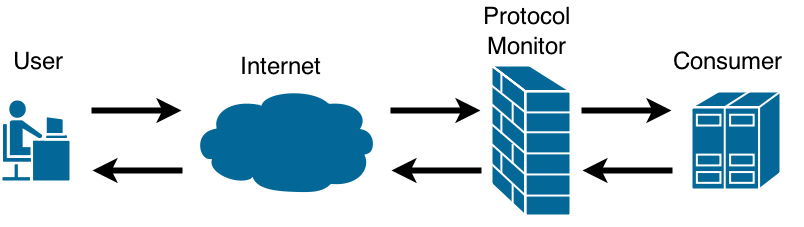
\includegraphics[scale=0.45]{images/architecture/ArchitectureFigure1.png} 
	\caption{Logical View of the architecture}
	\label{fig:ArchitectureFigure1}
\end{figure}
Figure \ref{fig:ArchitectureFigure1} shows the overall design for our concept. Users must connect through the internet to reach the Consumer. A Consumer is the entity that ``consumes'' the messages\footnote{A message is used to represent a package being sent from one client to the other} that get sent from the Protocol Monitor (PM). A message that goes through the PM must be the expected outcome of the protocol.

The PM is drawn as a firewall because it will act in the same way as a firewall does: it has rules that govern what messages are allowed to pass through. The rules contained within the PM will be defined by our DSL.

If a message is attempted to be sent or received and it breaks the protocol, the connection must be terminated. Attempting to repair the connection would prove to be difficult as there could be many reasons for a protocol to fail. Implementing fallbacks for all the various reasons could be to cumbersome of a task. Closing the connection is the simplest solution as it alerts both parties that the protocol has ended. Before the connection is closed, the consumer should have the option of sending a error message to the client allowing them to understand the reason the connection was closed.

%There should however be some form of construct that allows for a protocol to branch. This could be added to facilitate the use %%of multiple versions of a protocol in production.

At a later stage we will need to decide at what level the PM ensures that a protocol is obeyed. For simpler protocols we should be able to guaranty full protocol compliance. This becomes much harder to achieve in the case of when a consumer is expecting to receive an encrypted value and that value must have certain properties. For the PM to be able to handle these types of events, it must have the means to decrypt the message.

\subsubsection{Protocol Monitor}
In order for the architecture to function as we have described, the PM requires certain features. First, it must be able to know if a message received/sent is what the protocol expects. For this to happen the PM must know the state the protocol is in. This state must contain the means of verifying if a new message is expected. The second requirement is that it must be able to act appropriately for the messages received. This includes passing messages along to the users/consumers and also being able to terminate a connection.

The task of the PM is to forward and validate messages it receives. For it to validate these messages, it must also contain a state. Defining the state will be the task of the DSL. Defining such a protocol capable of containing a fluctuating state needs to be as effortless as possible. The syntax should also be concise so that reasoning about how the protocol operates is obvious.

\subsubsection{Consumer}
With our definition of what responsibilities the PM has, we can safely assume that all messages received by the consumer are expected. This means that it will not receive any messages that the protocol has not already dictated it should receive. This will remove a lot of error handling code in the implementation as the PM will take care of those. The only error that will need to be dealt with is when the protocol breaks.  


\subsubsection{Component mapping}
The task for the Protocol Monitor, Consumer and, optionally, the Client can be all implemented as actors as shown in figure \ref{fig:ArchitectureMapping}. The ``Client'' does not need to be implemented as an actor. Its only requirement is that it must obey the protocol. The client side could for example be someone using telnet or a web browser to communicate with a consumer/server.

This solution will allow the ``Consumer'' to create additional actors in a hierarchy beneath itself. This would allow for more concurrency and distribute the workload and state throughout a system.
\begin{figure}[h]
	\centering
	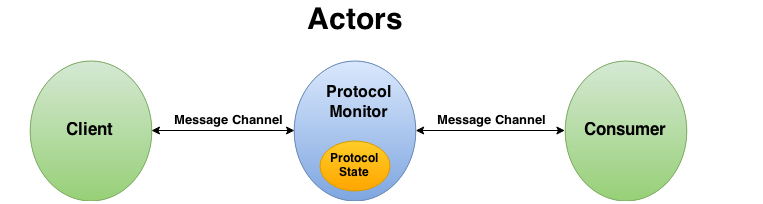
\includegraphics[scale=0.45]{images/architecture/ArchitectureMapping.png} 
	\caption{Representation of our Actors}
	\label{fig:ArchitectureMapping}
\end{figure}
We decided not to implement the ``Protocol State'' as a actor for a single reason. When the PM passes a message to be validated by the ``Protocol State'', it would be available to process new messages in its mailbox. This could potentially lead to race conditions occurring in a system. For now we will embed the state within the PM, but implementing the protocol state as an actor would certainly have a great advantage.

We have discussed how the PM will use the protocol state to determine its actions. What we now need is the ability to define such a state that can be used by the PM.

% arch end


\subsection{Defining a protocol}
One possible way of defining a protocol is to use the syntax shown below. This form of syntax is often used when discussing Session Types. They contain the direction of communication and the type of the message. 
$$
\begin{multlined}
Client \Rightarrow Server : Type \\ 
Server \Rightarrow Client : Type \\
end
\end{multlined}
$$
In this protocol the client sends a message to a server. The message that the server receives is to be of a certain type. Examples are: Integers, Strings, Objects etc. After the server has sent its last message, the protocol is over. 
A simple server that simply repeats the messages it receives, an echo server, would be defined in the following way:
$$
\begin{multlined}
Client \Rightarrow Server : String \\ 
Server \Rightarrow Client : String \\
end
\end{multlined}
$$
There is one undesired feature here however. When we reach the end, the connection is closed and we will need to re-establish a connection to send additional messages.
\subsubsection{Looping protocols}
Here we wish to once again implement a echo server. To avoid the user needing to reconnect for each message, we need to provide a way of looping the protocol. One approach would be to have a special case where we tell the protocol to go back to a previously defined step.
$$
\begin{multlined}
Client \Rightarrow Server : String \\ 
Server \Rightarrow Client : String \\ 
goto \rightarrow 0 \\
end
\end{multlined}
$$
When our Protocol Monitor now reaches the ``goto'' step, it should return back to step 0 of the protocol. This solution would however quickly become confusing if the number of goto steps was to increase. It is also not easy to know if the index begins on ``0'' or ``1''.
Also the the definition can become quite verbose when creating longer protocols. Another issue is that the state of both the ``Client'' and ``Server'' is mutated at each line.

\subsubsection{Implementation in Scala}
In Scala, we can create a syntax that is very similar to the session type syntax shown above. In the following example we will create two end-points, a client and a server. They will be used to define an echo server. First we need to create an instance of a object which has methods for sending, receiving and looping. For this purpose we have created the class ``ProtocolBuilder''. It contains the necessary functions and attributes needed for defining our protocol.
%[style=myScalastyle]
\begin{lstlisting}[style=myScalastyle]
 val client = new ProtocolBuilder()
 val server = new ProtocolBuilder()
\end{lstlisting}
Once they are created, we can begin to define our protocol.
\begin{lstlisting}[style=myScalastyle]
 client sends(server, aString)
 server sends(client, aString)
 server gotoStep 0
 client gotoStep 0 
\end{lstlisting}
The first and most obvious change is that we have dropped the arrow syntax in favour of ``sends'' and ``receives''. Although Scala can support such operators, it would not improve readability and would be difficult to type.

The second major change is that we are not using the type ``String'', but ``aString''. We will discuss this later is section {\ref{sec:validator} Validator}, but for now we will assume that ``aString'' is a validation on that the message is a string.   
\\\\
The main concern with this code is that we must define both the client and server side for each send and receive call. In a real implementation, we would only need to focus on one single end-point. By knowing one end of the protocol, we can construct the opposite protocol. In addition, Scala would allow us to omit the parentheses to increase readability, but not when we have two input parameters.
\\\\
Taking the above concerns into consideration, we propose a syntax that avoids this mutability and is less redundant. 

\subsubsection{Our protocol specification syntax}
The following shows the syntax in our DSL for defining a echo client and server.

\begin{lstlisting}[style=myScalastyle]
 val endpoint = new ProtocolBuilder()
 val client  = endpoint sends aString receives aString
 val server  = endpoint receives aString sends aString
\end{lstlisting}
We have removed mutability by making all calls to ``sends'' or ``receives'' return a new instance of a ProtocolBuilder(), this allows us to chain multiple send and receive in one line. This is very similar to the Builder pattern, hence the name.

As the value ``endpoint'' is never mutated, we can reuse the endpoint and be assured that it is always a blank starting point for us to use. 

To add a loop to the protocol, we add a call to ``loop()'' at the end.
\begin{lstlisting}[style=myScalastyle]
 val client = endpoint sends aString receives aString loop()
\end{lstlisting}
When the protocol state reaches loop(), it will return the state to the first defined step, in this case ``sends aString'' 

Another feature that we have added is that sometimes the order of messages is irrelevant. For example in a chat application, we want the participants to be able to send and receive in any possible order. For allowing this we have implemented the method ``anyone'' that represents being the sender or receiver of the current message is unimportant.

Although protocols are meant to be easy and not contain any complex branching, we have added features that would allow for such protocols. We may want to allow the usage of different versions of a protocol or other similar reasons.
\begin{lstlisting}[style=myScalastyle]
    val branchTest = Branch(input =>
      if (input forall Character.isDigit) IntegerProtocol
      else StringProtocol
    )
    val branching = endpoint branchOn branchTest
\end{lstlisting}
Branch takes an input and returns a ProtocolBuilder depending on the input. In our example we test if the all the characters in the input are digits. If they are, we return the IntegerProtocol, else we return the StringProtocol. Then finally we use our branch by calling ``branchOn'' and passing in our branch. 

% rename to Wrapper/
\subsection{Validator}
\label{sec:validator}
For the task of verifying if a message is of the expected type, we have created a class Validator. Validator is a class that contains a single method, ``validate''. This method contains the logic for testing if a message is of the correct type and expected value. The ``validate'' methods signature is as follows:
\begin{lstlisting}[style=myScalastyle]
    validate: String => Either[ValidationError, Any]
\end{lstlisting}
We will briefly explain this construct as it is a 
\begin{description}
 \item[validate] is the name of the method
 \item[String] is the input type for the method
 \item[=>] Given the previous input, return the following
 \item[Either\lbrack Left, Right\rbrack] Either return either a left or right value.
 \item[ValidationError] Left value is of type ValidationError
 \item[Any] Right value is of type Any. Any is, what its name suggest, a type that can return anything.
\end{description}
The main point to extract from this definition is the ``Either'' type. For the Either type, a ``Left'' value is considered undesired while the ``Right'' value is the desired one. In our case we set the undesired case to be ValidationError. Validation Error contains two arguments, a String and an optional Exception. The thought is to set the value of the String to an easy to understand message that will tell us what and where something went wrong. The exception will provide us with the details of why the error occurred. The ``Right'' value allows us to return an ``Any'' type of object. The object wrapped inside the Right object will be delivered directly to the Consumer. 

To show the simplicity of defining such Validators we will show some examples. First we will create a validator the verifies that a message can be converted to a String. The input of the ''validator`` is a string, so the message must be valid.
\begin{lstlisting}[style=myScalastyle]
  // Return input inside a Right()
  val aString = new Validator(input => Right(input))
  // Wrap input inside Username
  val aUsername = new Validator(input => Right(Username(input)))
\end{lstlisting}
As the input of the validator is a String, that means there is no way the validation can fail or be invalid. This allows us to avoid the need of including a ``Left'' value. To help with pattern matching, we can easily wrap this value inside a class. As shown in the value ``aUsername'' that wraps a string into a Username object.

We can also create more complex Validators that make more complex evaluation of a message. Here we can check if a message can fulfil the requirements of being a ``special number''.
\begin{lstlisting}[style=myScalastyle]
  val aSpecialNumber = new Validator(input => try {
    val number = input.toInt
    if(isSpecialNumber(number) {
        Right(SpecialNumber(number))
    } else {
        Left("Received message is not a SpecialNumber") 
    }
  } catch {
    case e: Exception =>
      Left(ValidationError("Received message is not an Integer", e) )
  })
\end{lstlisting}
The method ``isSpecialNumber'' does not need to be defined inside the validator. This is because Scala supports closures. They allow us to reference methods or variables outside the current local scope.

\subsubsection{Testing Validators}
One of the key features that was desired when designing the Validators was making them ligthweight and easily testable. In the case of our ``aSpecialNumber'' validator defined above we can quickly see all posible outputs from this Validator.
\begin{itemize}
  \item Right(SpecialNumber(number))
  \item Left("Received message is not a SpecialNumber") 
  \item Left(ValidationError("Received message is not an Integer", e))
\end{itemize}
The bare minimum should be writing tests for all three of these return cases. How many tests you create depends on how critical that validator is, but a test for each return type and edge cases should be more than sufficient for most.

\subsubsection{Encrypted  message validation}
When a message is encrypted, a validator will have no way to determine if it is valid. To do so, it would need to acquire the secret key that can decrypt the message. The secret key will only be available from the consumer. If we want to validate encrypted messages we can use the case class DelayedValidation.
 
\begin{lstlisting}[style=myScalastyle]
case class DelayedValidation(input: String, validator: Validator)
\end{lstlisting}

DelayedValidator has two attributes, a string and a validator. The string is the encrypted message and the Validator is going to validate the decrypted input. Once the consumer receives a DelayedValidator message it will decrypt the input and pass it back to the Protocol Monitor. The Protocol Monitor will then verify whether the message is valid. This provides us with consistency as it is always the PM that handles validation of messages. The DelayedValidation will also be useful in the cases where you accidentally send unencrypted values that should be encrypted. As the the attempt to decrypt a value that is not encrypted will throw an exception, we will not send it and stop the protocol.
   
%Ultimately we will need decide whether we should be able to define conditional steps. For example in the Diffie-Hellman-Merkle protocol, the secure public key must be agreed by both parties. If one client  
%

%loose coupling with protocol. no inheritance

\subsection{Protocol Monitor}
The Protocol Monitor tasks have been described in the previous sections. In this section we will briefly explain how our PM solution works.
\subsubsection{Startup}
To create an instance of a PM we require 3 things, two message channels and the protocol definition. The message channels are for communication with the client and consumer. These are both implemented as actors. 

Once the PM has been started, it sends an ``initiation'' message to the consumer. This will allow the consumer to be the one that begins the communication or to initialize resources needed.

%\subsubsection{Message forwarding}
%When the PM receives a message it will verify it is valid before sending it further. The PM will not %read the data inside these messages, it will only check whether it is a Left or Right value. 
%This is discussed in section \ref{sec:validator} Validator on page \pageref{sec:validator}.
\subsubsection{Ending the connection}
When the client disconnects, we tell the Consumer that we that we are done by sending a ``ProtocolEnded(reason)''. Here the value ``reason'' will represent why the connection ended, either the protocol finished or there was an error.

%Talk about how the PM works... How it communicates with the Connection and Consumer. + Initiation, +ErrorHandling, +Connection shutdown
%




